% !TeX program = lualatex
\documentclass[11pt,a4paper]{article}
\usepackage{szzmaterial}
\usetikzlibrary{calc,positioning,arrows.meta,shapes.geometric}
\setlist[enumerate]{nosep,leftmargin=2.1em}
\setlist[itemize]{nosep,leftmargin=1.8em}

\szztitul{Diskrétní matematika}{M3}{NDMI002 (Diskrétní matematika), NDMI011 (Kombinatorika a grafy 1)}

\newcommand{\Mcal}{\mathcal{M}}
\newcommand{\eqcl}[1]{[#1]}

\begin{document}
\maketitle
\tableofcontents
\bigskip

\section*{Úvod}
\addcontentsline{toc}{section}{Úvod}

Tento materiál pokrývá okruh \textbf{M3 -- Diskrétní matematika} (předměty NDMI002 \emph{Diskrétní matematika} a NDMI011 \emph{Kombinatorika a grafy 1}). Výklad jádra okruhu (relace, uspořádání, funkce, kombinatorické počítání a princip inkluze a exkluze) stojí na zápiscích T.~Slámy z přednášky doc.~Martina Mareše a na učebnici J.~Matouška a J.~Nešetřila \emph{Kapitoly z diskrétní matematiky} (v anglickém vydání \emph{Invitation to Discrete Mathematics}), kterou jako literaturu k~oběma předmětům doporučují jejich přednášející. Hallovu větu o systému různých reprezentantů uvádíme podle skript T.~Vally a J.~Matouška \emph{Kombinatorika a grafy I} (NDMI011). Značení a hloubka odpovídají kurzu pro informatiky.

U \emph{principu inkluze a exkluze} a \emph{Hallovy věty} požadavky okruhu výslovně uvádějí důkaz (resp.\ princip důkazu), proto je dokazujeme. Ostatní věty uvádíme \emph{se zněním}, doplněné intuicí a krátkými odvozeními tam, kde pomáhají pochopení. Do výkladu jsou zařazeny řešené reálné otázky SZZ z let 2022--2026; všechny otázky k okruhu jsou pohromadě v samostatném dokumentu \emph{Příklady otázek}. Použité zdroje jsou uvedeny na konci.

\medskip
\noindent\textbf{Značení.} Množiny značíme velkými písmeny $X,Y,A,B$, jejich velikost $|X|$. Kartézský součin je $X\times Y=\{(x,y):x\in X,\ y\in Y\}$, potenční množina (množina všech podmnožin) $2^X$, množina všech $k$-prvkových podmnožin $\binom{X}{k}$. Binární relaci píšeme $R$ a fakt $(x,y)\in R$ zkráceně $xRy$. Funkci (zobrazení) píšeme $f\colon X\to Y$. Symbolem $[n]$ míníme $\{1,2,\dots,n\}$, faktoriál $n!=1\cdot2\cdots n$ (s $0!=1$) a kombinační číslo $\binom{n}{k}$. Uspořádání značíme $\le$ (ostrou variantu $<$), částečně uspořádanou množinu (ČUM) dvojicí $(X,\le)$.

% ============================================================
\section{Relace, ekvivalence, rozkladové třídy}

Relace zachycuje vztah mezi prvky: kteří jsou \uv{ve vztahu} a kteří ne. Formálně je to prostě podmnožina kartézského součinu, tedy množina těch dvojic, které ve vztahu jsou.

\begin{definice}[Binární relace]
\emph{Binární relace} mezi množinami $X$ a $Y$ je libovolná podmnožina $R\subseteq X\times Y$. Je-li $X=Y$, mluvíme o \emph{relaci na množině $X$}. Místo $(x,y)\in R$ píšeme $xRy$.
\end{definice}

\begin{poznamka}
Speciální relace na $X$: \emph{prázdná} $\emptyset$ (nic s ničím), \emph{univerzální} $X\times X$ (vše se vším) a \emph{diagonální (identická)} $\Delta_X=\{(x,x):x\in X\}$ (každý prvek jen sám se sebou). K relaci $R$ definujeme \emph{inverzní} relaci $R^{-1}=\{(y,x):(x,y)\in R\}$ a ke dvojici relací $R\subseteq X\times Y$, $S\subseteq Y\times Z$ jejich \emph{složení} $R\circ S=\{(x,z):\exists y\in Y,\ xRy\wedge ySz\}$.
\end{poznamka}

\begin{intuice}
Relaci na konečné $X$ lze vidět dvěma způsoby. Jako \emph{matici} $|X|\times|X|$ nul a jedniček (na pozici $(x,y)$ je $1$, právě když $xRy$): diagonální relaci pak odpovídají jedničky na hlavní diagonále. Nebo jako \emph{orientovaný graf} na vrcholech $X$, kde šipka $x\to y$ vede právě pro $xRy$. Vlastnosti relací níže se hezky čtou na grafu.
\end{intuice}

\begin{definice}[Vlastnosti binární relace na $X$]
Relace $R$ na $X$ je
\begin{enumerate}[label=(\arabic*)]
  \item \emph{reflexivní}, pokud $\forall x\in X:\ xRx$;
  \item \emph{symetrická}, pokud $\forall x,y\in X:\ xRy\Rightarrow yRx$;
  \item \emph{antisymetrická}, pokud $\forall x,y\in X:\ (xRy\wedge yRx)\Rightarrow x=y$;
  \item \emph{tranzitivní}, pokud $\forall x,y,z\in X:\ (xRy\wedge yRz)\Rightarrow xRz$.
\end{enumerate}
\end{definice}

\begin{intuice}
Na grafu: \emph{reflexivita} = u každého vrcholu smyčka; \emph{symetrie} = každá šipka je obousměrná ($R^{-1}=R$); \emph{antisymetrie} = mezi dvěma různými vrcholy nevedou šipky oběma směry; \emph{tranzitivita} = vede-li cesta $x\to y\to z$, vede i přímá zkratka $x\to z$. Antisymetrie nezakazuje smyčky -- omezuje jen dvojice \emph{různých} prvků.
\end{intuice}

\begin{center}
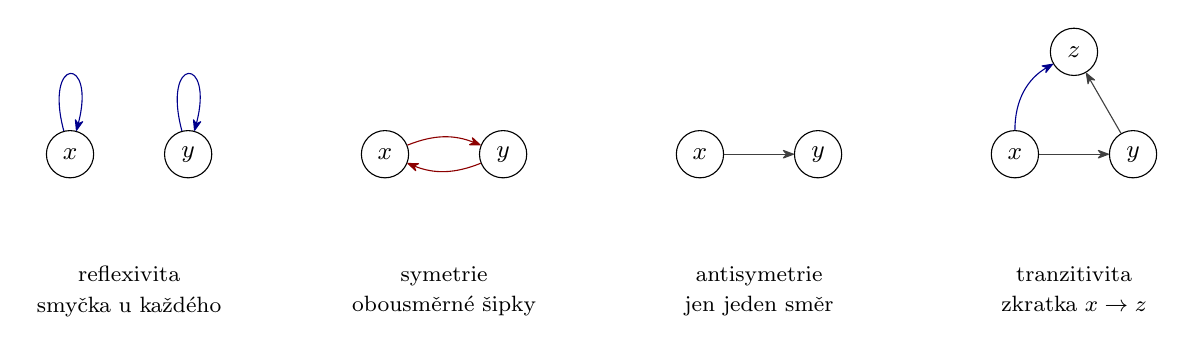
\begin{tikzpicture}[scale=1,>={Stealth[round]},font=\small,
  every loop/.style={min distance=6mm,looseness=16},
  vert/.style={circle,draw,minimum size=6mm,inner sep=0pt,font=\small}]
  % --- panel 1: reflexivita ---
  \begin{scope}[xshift=0cm]
    \node[vert] (a1) at (0,0) {$x$};
    \node[vert] (a2) at (1.5,0) {$y$};
    \draw[->,blue!55!black] (a1) edge[loop above] (a1);
    \draw[->,blue!55!black] (a2) edge[loop above] (a2);
    \node[below=1.3cm,align=center] at (0.75,0) {\footnotesize reflexivita\\\footnotesize smyčka u~každého};
  \end{scope}
  % --- panel 2: symetrie ---
  \begin{scope}[xshift=4cm]
    \node[vert] (b1) at (0,0) {$x$};
    \node[vert] (b2) at (1.5,0) {$y$};
    \draw[->,red!55!black,bend left=22] (b1) to (b2);
    \draw[->,red!55!black,bend left=22] (b2) to (b1);
    \node[below=1.3cm,align=center] at (0.75,0) {\footnotesize symetrie\\\footnotesize obousměrné šipky};
  \end{scope}
  % --- panel 3: antisymetrie ---
  \begin{scope}[xshift=8cm]
    \node[vert] (c1) at (0,0) {$x$};
    \node[vert] (c2) at (1.5,0) {$y$};
    \draw[->,black!75] (c1) to (c2);
    \node[below=1.3cm,align=center] at (0.75,0) {\footnotesize antisymetrie\\\footnotesize jen jeden směr};
  \end{scope}
  % --- panel 4: tranzitivita ---
  \begin{scope}[xshift=12cm]
    \node[vert] (d1) at (0,0) {$x$};
    \node[vert] (d2) at (1.5,0) {$y$};
    \node[vert] (d3) at (0.75,1.3) {$z$};
    \draw[->,black!75] (d1) to (d2);
    \draw[->,black!75] (d2) to (d3);
    \draw[->,blue!55!black,bend left=30] (d1) to (d3);
    \node[below=1.3cm,align=center] at (0.75,0) {\footnotesize tranzitivita\\\footnotesize zkratka $x\to z$};
  \end{scope}
\end{tikzpicture}\\[-0.5mm]
\end{center}

\begin{poznamka}
Antisymetrie z definice výše je tzv.\ \emph{slabá} antisymetrie: obousměrnou dvojici zakazuje jen pro \emph{různé} prvky, smyčku $xRx$ povoluje. Ekvivalentně $\forall x,y\in X,\ x\neq y:\ xRy\Rightarrow\neg\,yRx$. Vynecháme-li podmínku $x\neq y$, dostaneme \emph{silnou} (ostrou) antisymetrii, též \emph{asymetrii}: $\forall x,y\in X:\ xRy\Rightarrow\neg\,yRx$ -- ta navíc vylučuje i smyčky (je tedy ireflexivní). Slabou antisymetrii používá \emph{neostré} uspořádání $\le$ (reflexivní), asymetrie odpovídá \emph{ostrému} uspořádání $<$ (ireflexivní). Označení \uv{(slabě) antisymetrická} v příkladech níže míní právě tuto slabou variantu.
\end{poznamka}

\subsection{Ekvivalence a rozkladové třídy}

Některé relace vyjadřují \uv{stejnost v nějakém ohledu} (stejný zbytek po dělení, stejná barva). To jsou ekvivalence a my ukážeme, že přesně odpovídají rozkladům množiny na disjunktní části.

\begin{definice}[Ekvivalence a třída ekvivalence]
Relace $R$ na $X$ je \emph{ekvivalence}, je-li reflexivní, symetrická a tranzitivní. Pro $x\in X$ je \emph{třída ekvivalence} prvku $x$ množina $\eqcl{x}_R=\{y\in X:xRy\}$.
\end{definice}

\begin{definice}[Rozklad množiny]
\emph{Rozklad} množiny $X$ je systém neprázdných, navzájem disjunktních podmnožin $X$, jejichž sjednocením je celé $X$. Jednotlivé podmnožiny se nazývají \emph{třídy} rozkladu.
\end{definice}

\begin{veta}[Ekvivalence a rozklady si odpovídají]
Nechť $R$ je ekvivalence na $X$. Pak třídy $\eqcl{x}_R$ tvoří rozklad množiny $X$, tj.
\begin{enumerate}[label=(\arabic*)]
  \item každá třída je neprázdná a $x\in\eqcl{x}_R$;
  \item pro libovolná $x,y$ je buď $\eqcl{x}_R=\eqcl{y}_R$, nebo $\eqcl{x}_R\cap\eqcl{y}_R=\emptyset$.
\end{enumerate}
Naopak každý rozklad $X$ definuje ekvivalenci (\uv{být ve stejné třídě}) a tato dvě přiřazení jsou navzájem inverzní. Ekvivalence na $X$ tedy odpovídají jedna ku jedné rozkladům $X$.
\end{veta}

\begin{intuice}
Bod (1) je reflexivita. Klíčový bod (2) říká, že třídy se nepřekrývají \uv{napůl}: buď splynou, nebo jsou disjunktní. Důvod: leží-li $z$ ve dvou třídách $\eqcl{x}$ i $\eqcl{y}$, pak $xRz$ a $zRy$, takže ze symetrie a tranzitivity $xRy$, a obě třídy jsou stejné. Ekvivalence a rozklad jsou tedy jen dva pohledy na totéž.
\end{intuice}

\begin{priklad}[Typické ekvivalence]
Kongruence modulo $n$: $x\sim y\iff n\mid(x-y)$ na $\mathbb{Z}$ má $n$ tříd (zbytkové třídy $0,1,\dots,n-1$). Relace \uv{mít stejnou velikost} na podmnožinách dané množiny. Naopak \uv{být nesoudělný} ekvivalence není (není tranzitivní: $2$ a $3$, $3$ a $4$, ale $2$ a $4$ ne).
\end{priklad}

\noindent Následující reálná otázka kombinuje definici ekvivalence, počítání ekvivalencí a konstrukci relace s předepsanými vlastnostmi. Počet ekvivalencí spočteme rozborem tvarů rozkladu (díky předchozí větě ekvivalence $=$ rozklady).

\begin{priklad}[SZZ podzim 2025 č.~4: Binární relace] \szzotazka{podzim 2025}{4}{Binární relace}\par
\textbf{Zadání.}
\begin{enumerate}[label=(\arabic*)]
  \item Definujte podmínky, které musí splňovat binární relace $R$ na neprázdné množině $X$, aby byla ekvivalencí (pomocí kvantifikátorů a logických spojek).
  \item Pro $X=\{a,b,c,d\}$ určete, kolik různých ekvivalencí na $X$ existuje.
  \item Pro $X=\{a,b,c,d\}$ najděte relaci, která je tranzitivní, ale není symetrická ani (slabě) antisymetrická, a zdůvodněte to. (Antisymetrií se zde míní $\forall x,y\in X:(xRy\wedge yRx)\Rightarrow x=y$.)
\end{enumerate}

\textbf{Řešení.}
\begin{enumerate}[label=(\arabic*)]
  \item $R$ je ekvivalence, právě když je
    \begin{itemize}
      \item reflexivní: $\forall x\in X:\ (x,x)\in R$,
      \item symetrická: $\forall x,y\in X:\ (x,y)\in R\Rightarrow(y,x)\in R$,
      \item tranzitivní: $\forall x,y,z\in X:\ \big((x,y)\in R\wedge(y,z)\in R\big)\Rightarrow(x,z)\in R$.
    \end{itemize}
  \item \textbf{Rozklady po tvarech.} Ekvivalence na $X$ odpovídají rozkladům $X$, počítáme tedy rozklady $4$-prvkové množiny podle tvaru (velikostí tříd):
    \[
    \begin{array}{lll}
      \text{tvar } 4: & \text{1 blok}, & 1\ \text{rozklad},\\
      \text{tvar } 3+1: & \text{vybíráme samotný prvek } \binom{4}{1}, & 4,\\
      \text{tvar } 2+2: & \text{rozdělení na dvojice } \tfrac12\binom{4}{2}, & 3,\\
      \text{tvar } 2+1+1: & \text{vybíráme dvojici } \binom{4}{2}, & 6,\\
      \text{tvar } 1+1+1+1: & \text{samé singletony}, & 1.
    \end{array}
    \]
    Celkem $1+4+3+6+1=\boxed{15}$ ekvivalencí. (U tvaru $2+2$ dělíme dvěma, protože $\binom42=6$ započítává každou dvojici dvojic dvakrát.)
  \item Například $R=\{(a,a),(a,b),(b,a),(b,b),(c,d)\}$.\par
    \textbf{Tranzitivita.} Jediné dvojice, které na sebe navazují, jsou uvnitř bloku $\{a,b\}$ (ten je úplný, takže každá zkratka už v~$R$ je) a u~$(c,d)$ žádná navazující dvojice $(d,\cdot)$ neexistuje.\par
    \textbf{Symetrie.} $(c,d)\in R$, ale $(d,c)\notin R$ -- není symetrická.\par
    \textbf{Antisymetrie.} $(a,b),(b,a)\in R$, přitom $a\neq b$ -- není (slabě) antisymetrická.
\end{enumerate}
\begin{center}
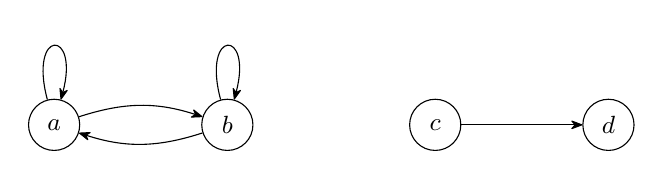
\begin{tikzpicture}[scale=1.1,>={Stealth[round]},every loop/.style={min distance=7mm,looseness=14},
  node distance=18mm,vert/.style={circle,draw,minimum size=6.5mm,inner sep=0pt,font=\small}]
  \node[vert] (a) at (0,0) {$a$};
  \node[vert] (b) at (2,0) {$b$};
  \node[vert] (c) at (4.4,0) {$c$};
  \node[vert] (d) at (6.4,0) {$d$};
  \draw[->] (a) edge[loop above] (a);
  \draw[->] (b) edge[loop above] (b);
  \draw[->,bend left=18] (a) to (b);
  \draw[->,bend left=18] (b) to (a);
  \draw[->] (c) to (d);
\end{tikzpicture}\obrpopis{Graf relace z bodu (3): blok $\{a,b\}$ je úplný (uvnitř tranzitivní), osamocená šipka $c\to d$ porušuje symetrii a obousměrná dvojice $a\leftrightarrow b$ porušuje antisymetrii.}
\end{center}
\end{priklad}

% ============================================================
\section{Částečná uspořádání}

Uspořádání zachycuje vztah \uv{být menší nebo roven} -- ne nutně mezi všemi dvojicemi. Formálně se liší od ekvivalence jen tím, že symetrii nahradíme antisymetrií.

\begin{definice}[Uspořádání]
Relace $\le$ na $X$ je \emph{(částečné) uspořádání}, je-li reflexivní, antisymetrická a tranzitivní; $(X,\le)$ pak nazýváme \emph{částečně uspořádaná množina} (ČUM). Uspořádání je \emph{lineární} (úplné), pokud jsou navíc každé dva prvky \emph{porovnatelné}: $\forall x,y\in X:\ x\le y\vee y\le x$. K~uspořádání $\le$ patří jeho \emph{ostrá} varianta $x<y\iff(x\le y\wedge x\neq y)$.
\end{definice}

\begin{center}
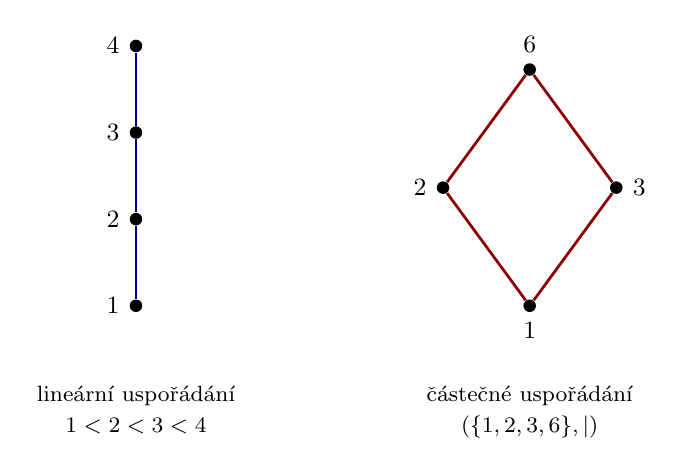
\begin{tikzpicture}[scale=1,vert/.style={circle,fill=black,inner sep=1.6pt},font=\small]
  % --- vlevo: linearni usporadani (retezec) ---
  \begin{scope}[xshift=0cm]
    \node[vert,label=left:{$1$}] (l1) at (0,0) {};
    \node[vert,label=left:{$2$}] (l2) at (0,1.1) {};
    \node[vert,label=left:{$3$}] (l3) at (0,2.2) {};
    \node[vert,label=left:{$4$}] (l4) at (0,3.3) {};
    \draw[blue!55!black,line width=1pt] (l1)--(l2)--(l3)--(l4);
    \node[below=0.9cm,align=center] at (0,0) {\footnotesize lineární uspořádání\\\footnotesize $1<2<3<4$};
  \end{scope}
  % --- vpravo: castecne usporadani (delitelnost {1,2,3,6}) ---
  \begin{scope}[xshift=5cm]
    \node[vert,label=below:{$1$}] (d1) at (0,0) {};
    \node[vert,label=left:{$2$}] (d2) at (-1.1,1.5) {};
    \node[vert,label=right:{$3$}] (d3) at (1.1,1.5) {};
    \node[vert,label=above:{$6$}] (d6) at (0,3) {};
    \draw[red!55!black,line width=1pt] (d1)--(d2);
    \draw[red!55!black,line width=1pt] (d1)--(d3);
    \draw[red!55!black,line width=1pt] (d2)--(d6);
    \draw[red!55!black,line width=1pt] (d3)--(d6);
    \node[below=0.9cm,align=center] at (0,0) {\footnotesize částečné uspořádání\\\footnotesize $(\{1,2,3,6\},\mid)$};
  \end{scope}
\end{tikzpicture}\obrpopis{Hasseovy diagramy. \emph{Lineární} (vlevo, řetězec $1<2<3<4$): každé dva prvky jsou porovnatelné, body leží svisle nad sebou. \emph{Částečné} (vpravo, dělitelnost na $\{1,2,3,6\}$): prvky $2$ a~$3$ nejsou porovnatelné (ani $2\mid3$, ani $3\mid2$), diagram má tvar kosočtverce.}
\end{center}

\begin{priklad}[Uspořádání]
$(\mathbb{R},\le)$ je lineární. $(2^X,\subseteq)$ (podmnožiny uspořádané inkluzí) a $(\mathbb{N},\mid)$ (dělitelnost) jsou jen částečná: $\{1\}$ a $\{2\}$ nejsou inkluzí porovnatelné, stejně jako $2$ a $3$ dělitelností.
\end{priklad}

\begin{definice}[Hasseův diagram]
\emph{Hasseův diagram} ČUM $(X,\le)$ je nákres, v němž $x$ leží níž než $y$, kdykoli $x<y$, a hranou spojujeme jen \emph{bezprostřední} dvojice: $x<y$ takové, že neexistuje $t$ s $x<t<y$. Ostatní vztahy doplní tranzitivita (čteme je \uv{po cestě vzhůru}).
\end{definice}

\begin{center}
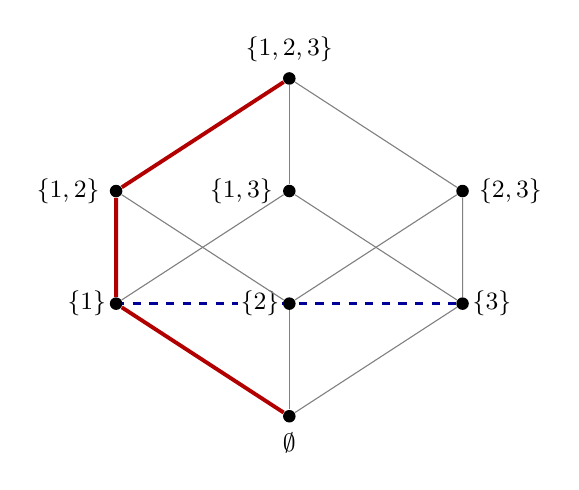
\begin{tikzpicture}[scale=1.1,vert/.style={circle,fill=black,inner sep=1.6pt},font=\small]
  % zvyraznit antiretezec (prostredni vrstva; pod uzly, popisky ji zakryji)
  \draw[blue!60!black,line width=1.2pt,dashed] (-2,1.3) -- (2,1.3);
  \node[vert,label=below:{$\emptyset$}] (e) at (0,0) {};
  \node[vert,label={[fill=white,inner sep=1pt]left:{$\{1\}$}}] (1) at (-2,1.3) {};
  \node[vert,label={[fill=white,inner sep=1pt]left:{$\{2\}$}}] (2) at (0,1.3) {};
  \node[vert,label={[fill=white,inner sep=1pt]right:{$\{3\}$}}] (3) at (2,1.3) {};
  \node[vert,label=left:{$\{1,2\}$}] (12) at (-2,2.6) {};
  \node[vert,label=left:{$\{1,3\}$}] (13) at (0,2.6) {};
  \node[vert,label=right:{$\{2,3\}$}] (23) at (2,2.6) {};
  \node[vert,label=above:{$\{1,2,3\}$}] (123) at (0,3.9) {};
  \foreach \a/\b in {e/1,e/2,e/3,1/12,1/13,2/12,2/23,3/13,3/23,12/123,13/123,23/123}
    \draw[gray] (\a) -- (\b);
  % zvyraznit retezec
  \draw[red!70!black,line width=1.4pt] (e)--(1)--(12)--(123);
\end{tikzpicture}\obrpopis{Hasseův diagram $(2^{\{1,2,3\}},\subseteq)$. Červeně řetězec $\emptyset\subset\{1\}\subset\{1,2\}\subset\{1,2,3\}$ (délka 4). Modře vyznačená vrstva $\{1\},\{2\},\{3\}$ je antiřetězec. Nejmenší prvek je $\emptyset$, největší $\{1,2,3\}$.}
\end{center}

\begin{definice}[Význačné prvky]
V ČUM $(X,\le)$ je prvek $a$
\begin{itemize}
  \item \emph{minimální}, neexistuje-li $x$ s $x<a$; \emph{maximální}, neexistuje-li $x$ s $a<x$;
  \item \emph{nejmenší}, je-li $\forall x\in X:\ a\le x$; \emph{největší}, je-li $\forall x\in X:\ x\le a$.
\end{itemize}
\end{definice}

\begin{intuice}
Rozdíl \uv{minimální} vs.\ \uv{nejmenší} je zásadní. \emph{Nejmenší} musí být porovnatelný se \emph{všemi} a být pod nimi -- proto je nejvýše jeden. \emph{Minimální} jen nesmí mít nic pod sebou, ale nemusí být s ostatními vůbec porovnatelný. V antiřetězci dvou prvků (žádné dva porovnatelné) jsou \emph{oba} minimální i maximální, a přitom není ani nejmenší, ani největší. Nejmenší prvek je vždy i minimální, opačně to neplatí.
\end{intuice}

\begin{definice}[Řetězec, antiřetězec, výška, šířka]
Podmnožina $C\subseteq X$ je \emph{řetězec}, jsou-li každé dva její prvky porovnatelné; je \emph{antiřetězec}, nejsou-li žádné dva její různé prvky porovnatelné. \emph{Výška} $v(X,\le)$ je velikost nejdelšího řetězce, \emph{šířka} $s(X,\le)$ je velikost nejdelšího antiřetězce.
\end{definice}

\begin{veta}[O dlouhém a širokém]
Pro každou konečnou ČUM $(X,\le)$ platí
\[
|X|\ \le\ v(X,\le)\cdot s(X,\le),
\]
tj.\ počet prvků nepřevýší součin výšky a šířky.
\end{veta}

\begin{intuice}
\uv{Buď je něco dlouhé (vysoký řetězec), nebo široké (velký antiřetězec) -- jinak se tolik prvků nevejde.} Myšlenka důkazu: množinu rozvrstvíme na patra minimálních prvků. Každé patro je antiřetězec (nejvýše $s$ prvků) a pater je nejvýše tolik, kolik měří nejdelší řetězec ($v$), protože každý prvek z $k$-tého patra je vrcholem řetězce délky $k$ jdoucího skrz všechna nižší patra.
\end{intuice}

\begin{proof}[Důkaz \textnormal{(nepovinný -- princip)}]
Položme $M_1=\{$minimální prvky $X\}$, $X_1=X\setminus M_1$, dále $M_2=\{$minimální prvky $X_1\}$ atd., dokud něco zbývá; vznikne rozklad $X=M_1\cup\dots\cup M_t$. Každé $M_i$ je antiřetězec (dva minimální prvky téže úrovně nemohou být porovnatelné), tedy $|M_i|\le s$. Je-li $a\in M_k$ pro $k\ge2$, pak $a$ leží v~$X_{k-2}$ (kde $X_0=X$), ale nebyl v~ní minimální (jinak by patřil do $M_{k-1}$). Pod $a$ tedy v~$X_{k-2}$ leží nějaký prvek, a protože je $X$ konečná, i nějaký minimální prvek $a_{k-1}\in M_{k-1}$ s~$a_{k-1}<a$; pokračováním dolů dostaneme řetězec $a_1<a_2<\dots<a_k=a$ délky $k$, proto $k\le v$. Tedy pater je nejvýše $v$ a
\[
|X|=\sum_{i=1}^{t}|M_i|\le t\cdot s\le v\cdot s.
\]
\end{proof}

\begin{center}
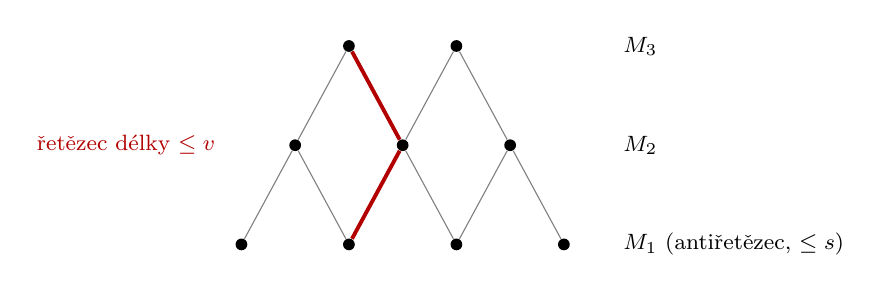
\begin{tikzpicture}[scale=1.05,vert/.style={circle,fill=black,inner sep=1.5pt},font=\small]
  % patra (antiretezce) M1 (dole) az M3 (nahore)
  \node[vert] (p1) at (0,0) {}; \node[vert] (p2) at (1.3,0) {}; \node[vert] (p3) at (2.6,0) {}; \node[vert] (p4) at (3.9,0) {};
  \node[vert] (q1) at (0.65,1.2) {}; \node[vert] (q2) at (1.95,1.2) {}; \node[vert] (q3) at (3.25,1.2) {};
  \node[vert] (r1) at (1.3,2.4) {}; \node[vert] (r2) at (2.6,2.4) {};
  % hrany (uspořádání)
  \draw[gray] (p1)--(q1) (p2)--(q1) (p2)--(q2) (p3)--(q2) (p3)--(q3) (p4)--(q3);
  \draw[gray] (q1)--(r1) (q2)--(r1) (q2)--(r2) (q3)--(r2);
  % popisky pater
  \node[anchor=west] at (4.5,0) {\footnotesize $M_1$ (antiřetězec, $\le s$)};
  \node[anchor=west] at (4.5,1.2) {\footnotesize $M_2$};
  \node[anchor=west] at (4.5,2.4) {\footnotesize $M_3$};
  % zvyrazneny retezec napric patry
  \draw[red!70!black,line width=1.4pt] (p2)--(q2)--(r1);
  \node[red!70!black,anchor=east] at (-0.2,1.2) {\footnotesize řetězec délky $\le v$};
\end{tikzpicture}\obrpopis{Rozvrstvení na patra minimálních prvků: každé patro je antiřetězec (vodorovně, $\le s$ prvků), červený řetězec protíná každé patro nejvýše jednou (proto $\le v$ pater), odtud $|X|\le v\cdot s$.}
\end{center}

\begin{poznamka}
Kontrola na obrázku výše: v $(2^{\{1,2,3\}},\subseteq)$ je výška $v=4$ (řetězec $\emptyset\subset\{1\}\subset\{1,2\}\subset\{1,2,3\}$) a šířka $s=3$ (největší antiřetězec, např.\ trojice jednoprvkových), takže $8=|X|\le v\cdot s=12$.
\end{poznamka}

\begin{priklad}[Aplikace: Erdős--Szekeres]
\textbf{Zadání.} Z věty o dlouhém a širokém odvoďte: každá posloupnost $n^2+1$ navzájem různých reálných čísel obsahuje rostoucí nebo klesající podposloupnost délky alespoň $n+1$.

\textbf{Řešení.} Na indexech $\{1,\dots,n^2+1\}$ definujme uspořádání $i\preceq j\iff(i\le j\ \wedge\ x_i\le x_j)$. (Reflexivita, antisymetrie i tranzitivita plynou z téhož pro $\le$ na obou složkách.) \emph{Řetězec} v $\preceq$ je rostoucí podposloupnost, \emph{antiřetězec} je klesající podposloupnost (rostoucí v indexu, ale klesající v hodnotě). Podle věty o dlouhém a širokém je $n^2+1=|X|\le v\cdot s$, takže $v\ge n+1$ nebo $s\ge n+1$ (jinak by $v\cdot s\le n^2$). To je hledaná podposloupnost délky $n+1$.
\end{priklad}

% ============================================================
\section{Funkce: typy a počty}

Funkce je speciální relace, ve které jde z každého prvku právě jedna šipka. Spočítáme, kolik je různých typů funkcí mezi konečnými množinami -- základní cvičení \uv{kombinatorického počítání}.

\begin{definice}[Funkce a její typy]
Relace $f\subseteq X\times Y$ je \emph{funkce (zobrazení)} $f\colon X\to Y$, pokud ke každému $x\in X$ existuje právě jedno $y$ s $(x,y)\in f$; píšeme $f(x)=y$. Funkce je
\begin{itemize}
  \item \emph{prostá (injektivní)}: $\forall x,x'\in X:\ x\neq x'\Rightarrow f(x)\neq f(x')$;
  \item \emph{na (surjektivní)}: $\forall y\in Y\ \exists x\in X:\ f(x)=y$;
  \item \emph{bijekce}: zároveň prostá a na ($\forall y\in Y$ existuje právě jedno $x$ s $f(x)=y$).
\end{itemize}
\end{definice}

\begin{center}
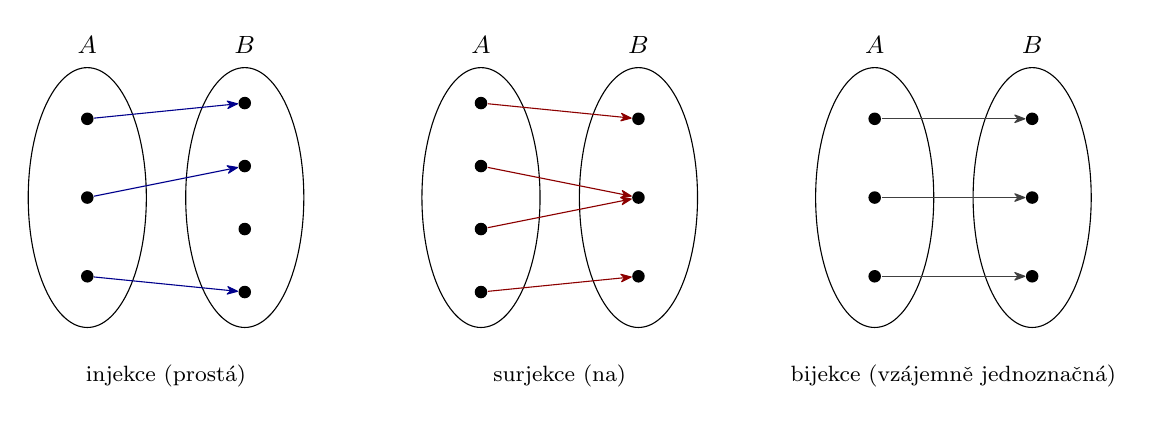
\begin{tikzpicture}[scale=1,>={Stealth[round]},font=\small,
  dot/.style={circle,fill=black,inner sep=1.6pt},
  ovalA/.style={draw,ellipse,minimum width=1.5cm,minimum height=3.3cm},
  ovalB/.style={draw,ellipse,minimum width=1.5cm,minimum height=3.3cm}]
  % --- panel 1: injekce ---
  \begin{scope}[xshift=0cm]
    \node[ovalA] at (0,0) {};
    \node[ovalB] at (2,0) {};
    \node[above=1.7cm] at (0,0) {$A$};
    \node[above=1.7cm] at (2,0) {$B$};
    \node[dot] (a1) at (0,1) {}; \node[dot] (a2) at (0,0) {}; \node[dot] (a3) at (0,-1) {};
    \node[dot] (b1) at (2,1.2) {}; \node[dot] (b2) at (2,0.4) {}; \node[dot] (b3) at (2,-0.4) {}; \node[dot] (b4) at (2,-1.2) {};
    \draw[->,blue!55!black] (a1) -- (b1);
    \draw[->,blue!55!black] (a2) -- (b2);
    \draw[->,blue!55!black] (a3) -- (b4);
    \node[below=2cm] at (1,0) {\footnotesize injekce (prostá)};
  \end{scope}
  % --- panel 2: surjekce ---
  \begin{scope}[xshift=5cm]
    \node[ovalA] at (0,0) {};
    \node[ovalB] at (2,0) {};
    \node[above=1.7cm] at (0,0) {$A$};
    \node[above=1.7cm] at (2,0) {$B$};
    \node[dot] (c1) at (0,1.2) {}; \node[dot] (c2) at (0,0.4) {}; \node[dot] (c3) at (0,-0.4) {}; \node[dot] (c4) at (0,-1.2) {};
    \node[dot] (d1) at (2,1) {}; \node[dot] (d2) at (2,0) {}; \node[dot] (d3) at (2,-1) {};
    \draw[->,red!55!black] (c1) -- (d1);
    \draw[->,red!55!black] (c2) -- (d2);
    \draw[->,red!55!black] (c3) -- (d2);
    \draw[->,red!55!black] (c4) -- (d3);
    \node[below=2cm] at (1,0) {\footnotesize surjekce (na)};
  \end{scope}
  % --- panel 3: bijekce ---
  \begin{scope}[xshift=10cm]
    \node[ovalA] at (0,0) {};
    \node[ovalB] at (2,0) {};
    \node[above=1.7cm] at (0,0) {$A$};
    \node[above=1.7cm] at (2,0) {$B$};
    \node[dot] (e1) at (0,1) {}; \node[dot] (e2) at (0,0) {}; \node[dot] (e3) at (0,-1) {};
    \node[dot] (g1) at (2,1) {}; \node[dot] (g2) at (2,0) {}; \node[dot] (g3) at (2,-1) {};
    \draw[->,black!75] (e1) -- (g1);
    \draw[->,black!75] (e2) -- (g2);
    \draw[->,black!75] (e3) -- (g3);
    \node[below=2cm] at (1,0) {\footnotesize bijekce (vzájemně jednoznačná)};
  \end{scope}
\end{tikzpicture}\obrpopis{Tři typy funkcí. \emph{Injekce} (prostá): různé vzory mají různé obrazy, v~$B$ smí zbýt nepokrytý prvek. \emph{Surjekce} (na): každý prvek $B$ je pokryt, ale dva prvky $A$ mohou mířit na týž. \emph{Bijekce} (vzájemně jednoznačná): prostá i na zároveň, prvky se párují $1{:}1$.}
\end{center}

\begin{veta}[Počty funkcí mezi konečnými množinami]
Nechť $|A|=a$ a $|B|=b$. Pak počet
\begin{enumerate}[label=(\arabic*)]
  \item \emph{všech} funkcí $A\to B$ je $\ b^{a}$;
  \item \emph{prostých} funkcí $A\to B$ je $\ b\,(b-1)\cdots(b-a+1)=\dfrac{b!}{(b-a)!}$ \ (pro $a\le b$, jinak $0$);
  \item \emph{bijekcí} $A\to B$ je $\ a!$ \ (jen je-li $a=b$, jinak $0$);
  \item \emph{surjekcí} $A\to B$ je $\ \displaystyle\sum_{k=0}^{b}(-1)^k\binom{b}{k}(b-k)^{a}$ (odvodíme v sekci \ref{sec:ie} principem inkluze a exkluze).
\end{enumerate}
\end{veta}

\begin{intuice}
(1) Každý z $a$ prvků poslat nezávisle na kterýkoli z $b$ -- $b\cdot b\cdots b=b^a$. (2) Aby byla prostá, ubývají možnosti: první prvek má $b$ cílů, druhý $b-1$ (jeden je obsazený) atd. (3) Bijekce $A\to A$ je právě prostá funkce $A\to A$, tedy $a(a-1)\cdots1=a!$. Speciálně počet podmnožin $X$ je $|2^X|=2^{|X|}$ -- podmnožiny odpovídají funkcím $X\to\{0,1\}$ (charakteristická funkce: $1$ pro prvky uvnitř).
\end{intuice}

\begin{priklad}[Počty funkcí]
\textbf{Zadání.} Kolik je funkcí, prostých funkcí a bijekcí z $A=\{1,2,3\}$ do $B=\{1,2,3,4\}$?

\textbf{Řešení.} Všech: $b^a=4^3=64$. Prostých: $4\cdot3\cdot2=24$. Bijekcí: $0$ (je $|A|\neq|B|$, bijekce neexistuje). Naopak prostých funkcí z $B$ do $A$ je $0$ (nelze $4$ různé prvky injektivně uložit do $3$).
\end{priklad}

\begin{priklad}[SZZ léto 2022 č.~4: Injekce a surjekce -- definice a počty] \szzotazka{léto 2022}{4}{Zobrazení (injekce, surjekce, počty)}\par
\textbf{Zadání.}
\begin{enumerate}[label=(\arabic*)]
  \item Definujte, kdy je zobrazení $f\colon X\to Y$ prosté (injektivní) a kdy \uv{na} (surjektivní).
  \item Pro $n\in\mathbb{N}$ určete, kolik existuje prostých zobrazení z $\{1,\dots,n\}$ do $\{1,\dots,2n\}$.
  \item Pro $n\in\mathbb{N}$ určete, kolik existuje zobrazení $\{1,\dots,2n\}$ na $\{1,\dots,n\}$ takových, že pro každé $k\in\{1,\dots,n\}$ existují právě dvě hodnoty $i,j$ s~$f(i)=f(j)=k$.
\end{enumerate}
\textbf{Řešení.}
\begin{enumerate}[label=(\arabic*)]
  \item $f$ je prosté: $\forall a,b\in X:\ f(a)=f(b)\Rightarrow a=b$ (různé vzory mají různé obrazy). $f$ je na: $\forall y\in Y\ \exists x\in X:\ f(x)=y$ (každý prvek $Y$ je obrazem).
  \item Po prvcích: první obraz má $2n$ možností, druhý $2n-1$, \dots, $n$-tý $n+1$, celkem $2n\cdot(2n-1)\cdots(n+1)=\frac{(2n)!}{n!}$.
  \item Jde o rozdělení $2n$ prvků do $n$ \emph{označených} dvojic; uspořádaných $2n$-tic je $(2n)!$, v každé z $n$ dvojic nezáleží na pořadí, tedy $\frac{(2n)!}{(2!)^n}=\frac{(2n)!}{2^n}$. (Kontrola $n=2$: prostých $4\cdot3=12=\frac{4!}{2!}$, takových surjekcí $\frac{4!}{2^2}=6$.)
\end{enumerate}
\end{priklad}

% ============================================================
\section{Permutace, kombinační čísla, binomická věta}

\subsection{Permutace}

\begin{definice}[Permutace, pevný bod]
\emph{Permutace} množiny $X$ je bijekce $p\colon X\to X$. Na $[n]$ značíme množinu všech permutací $S_n$. \emph{Pevný bod} permutace $p$ je prvek $x$ s $p(x)=x$.
\end{definice}

\begin{veta}[Počet permutací]
Permutací $n$-prvkové množiny je $\ n!=n(n-1)\cdots1$.
\end{veta}

\begin{intuice}
Permutace je prostá funkce $[n]\to[n]$, takže podle předchozí věty jich je $n(n-1)\cdots1=n!$ (první prvek má $n$ obrazů, druhý $n-1$, \dots). Permutaci lze rozložit na nezávislé \emph{cykly}; pevné body jsou právě cykly délky $1$. Počet permutací \emph{bez} pevného bodu spočteme v sekci~\ref{sec:ie} (problém šatnářky).
\end{intuice}

\subsection{Kombinační čísla}

\begin{definice}[Kombinační číslo]
Pro celá $0\le k\le n$ je \emph{kombinační číslo}
\[
\binom{n}{k}=\frac{n!}{k!\,(n-k)!}=\frac{n(n-1)\cdots(n-k+1)}{k!}.
\]
\end{definice}

\begin{veta}[Kombinační číslo počítá podmnožiny]
$\binom{n}{k}$ je počet $k$-prvkových podmnožin $n$-prvkové množiny, tj.\ $\big|\binom{X}{k}\big|=\binom{|X|}{k}$.
\end{veta}

\begin{intuice}
Uspořádaných $k$-tic různých prvků z $n$-prvkové $X$ je $n(n-1)\cdots(n-k+1)$ (prostá funkce $[k]\to X$). Každá $k$-prvková podmnožina dá $k!$ takových $k$-tic (jejím přerovnáním). Proto počet podmnožin je podíl $\frac{n(n-1)\cdots(n-k+1)}{k!}=\binom{n}{k}$.
\end{intuice}

\begin{veta}[Vztahy mezi kombinačními čísly]
Pro $0\le k\le n$ platí
\begin{enumerate}[label=(\arabic*)]
  \item symetrie: $\displaystyle\binom{n}{k}=\binom{n}{n-k}$;
  \item Pascalův vztah: $\displaystyle\binom{n}{k}=\binom{n-1}{k-1}+\binom{n-1}{k}$;
  \item součet řádku: $\displaystyle\sum_{k=0}^{n}\binom{n}{k}=2^{n}$;
  \item alternující součet: $\displaystyle\sum_{k=0}^{n}(-1)^k\binom{n}{k}=0$ (pro $n\ge1$).
\end{enumerate}
\end{veta}

\begin{intuice}
(1) Vybrat $k$ prvků \uv{dovnitř} je totéž jako vybrat $n-k$ \uv{ven}. (2) Zafixujme jeden prvek: $k$-prvkové podmnožiny ho buď neobsahují ($\binom{n-1}{k}$ způsobů), nebo obsahují a zbytek vybíráme z ostatních ($\binom{n-1}{k-1}$). To je pravidlo \uv{sčítání dvou čísel nad sebou} v Pascalově trojúhelníku. (3) Součet počtů podmnožin všech velikostí je počet všech podmnožin $2^n$. (4) Plyne dosazením $a=1,b=-1$ do binomické věty níže -- podmnožin sudé velikosti je stejně jako lichých.
\end{intuice}

\begin{center}
\begin{tikzpicture}[scale=0.68,font=\small]
  % rucne vypsane hodnoty (radky 0..5)
  \node at (0,0) {$1$};
  \node at (-0.9,-1) {$1$}; \node at (0.9,-1) {$1$};
  \node at (-1.8,-2) {$1$}; \node at (0,-2) {$2$}; \node at (1.8,-2) {$1$};
  \node at (-2.7,-3) {$1$}; \node at (-0.9,-3) {$3$}; \node at (0.9,-3) {$3$}; \node at (2.7,-3) {$1$};
  \node at (-3.6,-4) {$1$}; \node at (-1.8,-4) {$4$}; \node at (0,-4) {$6$}; \node at (1.8,-4) {$4$}; \node at (3.6,-4) {$1$};
  \node at (-4.5,-5) {$1$}; \node at (-2.7,-5) {$5$}; \node at (-0.9,-5) {$10$}; \node at (0.9,-5) {$10$}; \node at (2.7,-5) {$5$}; \node at (4.5,-5) {$1$};
  % sipky Pascalova pravidla: 4 a 6 (radek 4) -> 10 (radek 5, pozice k=2)
  \draw[->,red!70!black,thick] (-1.8,-4.25) -- (-1.05,-4.78);
  \draw[->,red!70!black,thick] (-0.1,-4.25) -- (-0.85,-4.78);
  \node[red!70!black] at (-0.9,-6.1) {\footnotesize $\binom{5}{2}=\binom{4}{1}+\binom{4}{2}$};
\end{tikzpicture}\obrpopis{Pascalův trojúhelník. Každé číslo je součtem dvou nad ním (Pascalův vztah); součet $n$-tého řádku je $2^n$.}
\end{center}

\subsection{Binomická věta}

\begin{veta}[Binomická věta]
Pro $n\in\mathbb{N}_0$ a libovolná $a,b$ (z komutativního okruhu, např.\ $\mathbb{R}$) platí
\[
(a+b)^{n}=\sum_{k=0}^{n}\binom{n}{k}a^{\,n-k}b^{\,k}.
\]
\end{veta}

\begin{intuice}
Roznásobujeme $n$ závorek $(a+b)$. Z~každé vybereme buď $a$, nebo $b$; výsledný člen s~právě $k$ vybranými $b$ je $a^{n-k}b^{k}$ a počet způsobů, jak vybrat oněch $k$ závorek dávajících $b$, je $\binom{n}{k}$. Sečtením přes $k$ dostaneme vzorec.
\end{intuice}

\begin{priklad}[Aplikace binomické věty]
\textbf{Zadání.} Odvoďte $\sum_{k=0}^n\binom nk=2^n$ a $\sum_{k=0}^n(-1)^k\binom nk=0$.

\textbf{Řešení.} Dosazením $a=b=1$: $(1+1)^n=\sum_k\binom nk 1^{n-k}1^k=\sum_k\binom nk$, tedy $2^n$. Dosazením $a=1,b=-1$: $(1-1)^n=0=\sum_k\binom nk(-1)^k$ (pro $n\ge1$). Druhý vztah říká, že podmnožin sudé velikosti je stejně jako lichých.
\end{priklad}

% ============================================================
\section{Princip inkluze a exkluze}\label{sec:ie}

Chceme spočítat velikost sjednocení množin, které se mohou překrývat. Sečíst velikosti nestačí (průniky se započtou víckrát); princip inkluze a exkluze je systematicky \uv{přičítá a odečítá}.

\begin{veta}[Princip inkluze a exkluze]
Pro konečné množiny $A_1,\dots,A_n$ platí
\[
\Big|\bigcup_{i=1}^{n}A_i\Big|
=\sum_{k=1}^{n}(-1)^{k-1}\!\!\sum_{\substack{I\subseteq[n]\\|I|=k}}\Big|\bigcap_{i\in I}A_i\Big|
=\sum_{\emptyset\neq I\subseteq[n]}(-1)^{|I|-1}\Big|\bigcap_{i\in I}A_i\Big|.
\]
Pro $n=2$ je to známé $|A_1\cup A_2|=|A_1|+|A_2|-|A_1\cap A_2|$.
\end{veta}

\begin{intuice}
\uv{Přičti jednotlivé, odečti dvojnásobně započtené průniky dvojic, přičti zpět trojic, \dots} Sudé průniky se odečítají, liché přičítají, aby každý prvek byl nakonec započten přesně jednou.
\end{intuice}

\begin{proof}[Důkaz (počítací).]
Ukážeme, že každý prvek $x\in\bigcup A_i$ je na obou stranách započten právě jednou. Vlevo jednou (je ve sjednocení). Vpravo: leží-li $x$ v právě $j$ množinách ($j\ge1$), pak $x\in\bigcap_{i\in I}A_i$ právě pro ty $I$, které jsou podmnožinami oněch $j$ množin; takových $I$ velikosti $k$ je $\binom{j}{k}$. Příspěvek $x$ vpravo je tedy
\[
\sum_{k=1}^{j}(-1)^{k-1}\binom{j}{k}
=-\sum_{k=1}^{j}(-1)^{k}\binom{j}{k}
=-\Big(\underbrace{\sum_{k=0}^{j}(-1)^k\binom{j}{k}}_{=(1-1)^j=0}-\,\binom{j}{0}\Big)
=-(0-1)=1.
\]
Obě strany tedy počítají každý prvek jednou.
\end{proof}

\begin{center}
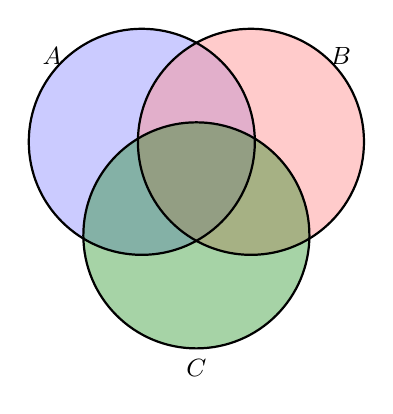
\begin{tikzpicture}[scale=0.99,font=\small]
  \def\rad{1.45}
  % tri symetricky rozmistene kruhy; poloprusvitna vypln -> prekryvy ztmavnou samy
  \fill[blue!45,fill opacity=0.45] (-0.7, 0.45) circle (\rad);
  \fill[red!45, fill opacity=0.45] ( 0.7, 0.45) circle (\rad);
  \fill[green!50!black,fill opacity=0.35] (0,-0.75) circle (\rad);
  \draw[thick] (-0.7, 0.45) circle (\rad);
  \draw[thick] ( 0.7, 0.45) circle (\rad);
  \draw[thick] ( 0,  -0.75) circle (\rad);
  \node at (-1.85, 1.55) {$A$};
  \node at ( 1.85, 1.55) {$B$};
  \node at ( 0,   -2.45) {$C$};
\end{tikzpicture}\obrpopis{Vennův diagram tří množin: $|A\cup B\cup C|=|A|+|B|+|C|-|A\cap B|-|A\cap C|-|B\cap C|+|A\cap B\cap C|$. Překryvy se nejdřív odečtou (jsou započteny dvakrát) a trojitý průnik se zpět přičte.}
\end{center}

\subsection{Použití (1): problém šatnářky}

\begin{priklad}[Problém šatnářky -- permutace bez pevného bodu]
\textbf{Zadání.} $n$ pánů odevzdá v šatně klobouky a šatnářka jim je vrátí náhodně, každému jeden. Jaká je pravděpodobnost, že \emph{nikdo} nedostane svůj klobouk? Ekvivalentně: kolik je permutací $D(n)$ na $[n]$ \emph{bez pevného bodu}?

\textbf{Řešení.}
Vrácení klobouků je náhodná permutace $\pi$; \uv{pán $i$ dostal svůj} znamená pevný bod $\pi(i)=i$. Spočteme \uv{špatné} permutace (alespoň jeden pevný bod). Pro $i\in[n]$ nechť $A_i=\{\pi\in S_n:\pi(i)=i\}$. Pak $|A_i|=(n-1)!$ (ostatních $n-1$ prvků libovolně) a obecně pro $i_1<\dots<i_k$ je $\big|\bigcap_{j}A_{i_j}\big|=(n-k)!$ (zafixujeme $k$ bodů).\par
\textbf{Inkluze--exkluze.}
\[
\Big|\bigcup_{i}A_i\Big|=\sum_{k=1}^{n}(-1)^{k-1}\binom{n}{k}(n-k)!
=\sum_{k=1}^{n}(-1)^{k-1}\frac{n!}{k!},
\]
takže permutací bez pevného bodu je
\[
D(n)=n!-\Big|\bigcup_i A_i\Big|=n!\sum_{k=0}^{n}\frac{(-1)^k}{k!}.
\]
\textbf{Limita.} Hledaná pravděpodobnost je $\dfrac{D(n)}{n!}=\sum_{k=0}^{n}\dfrac{(-1)^k}{k!}\xrightarrow[n\to\infty]{}\boxed{e^{-1}\approx0{,}368}$. Pozoruhodné je, že na počtu pánů skoro nezáleží.
\end{priklad}

\subsection{Použití (2): Eulerova funkce}

\begin{priklad}[Eulerova funkce $\varphi(n)$]
\textbf{Zadání.} $\varphi(n)$ je počet čísel $m\in[n]$ nesoudělných s $n$ (tj.\ $\gcd(n,m)=1$). Odvoďte vzorec pomocí prvočíselného rozkladu $n=p_1^{\alpha_1}\cdots p_r^{\alpha_r}$.

\textbf{Řešení.} \uv{Špatná} $m\le n$ (soudělná s $n$) jsou právě násobky některého z prvočísel $p_i$. Nechť $A_i=\{m\in[n]:p_i\mid m\}$; pak $|A_i|=\tfrac{n}{p_i}$ a obecně $\big|\bigcap_{j}A_{i_j}\big|=\tfrac{n}{p_{i_1}\cdots p_{i_k}}$ (násobky součinu příslušných prvočísel). Je $\varphi(n)=n-\big|\bigcup_i A_i\big|$, tedy principem inkluze a exkluze
\[
\varphi(n)=n\sum_{I\subseteq\{1,\dots,r\}}\frac{(-1)^{|I|}}{\prod_{i\in I}p_i}
=n\prod_{i=1}^{r}\Big(1-\frac{1}{p_i}\Big).
\]
Například $\varphi(12)=\varphi(2^2\cdot3)=12(1-\tfrac12)(1-\tfrac13)=12\cdot\tfrac12\cdot\tfrac23=4$ (čísla $1,5,7,11$).
\end{priklad}

\begin{intuice}
Roznásobení součinu $n\prod_i(1-\frac1{p_i})$ dá přesně střídavou sumu inkluze a exkluze: člen $\frac{(-1)^{|I|}n}{\prod_{i\in I}p_i}$ pro každou podmnožinu prvočísel $I$. (Požadavky M3 tuto funkci zmiňují slovy \uv{Eulerova funkce pro počet dělitelů}; míní se jí právě $\varphi$, tj.\ počet zbytkových tříd nesoudělných s~$n$.)
\end{intuice}

\subsection{Použití (3): počet surjekcí}

\begin{priklad}[Počet surjekcí]
\textbf{Zadání.} Spočtěte počet surjekcí (funkcí \uv{na}) z $a$-prvkové množiny $A$ na $b$-prvkovou množinu $B$.

\textbf{Řešení.} Spočteme \uv{špatné} funkce (nejsou na, tedy nějaký prvek $B$ vynechají). Pro $y\in B$ nechť $A_y=\{f\colon A\to B:\ y\notin f(A)\}$ (funkce vynechávající $y$). Pak $|A_y|=(b-1)^a$ (cílů je jen $b-1$) a obecně průnik $k$ takových množin (vynechání $k$ daných prvků) má velikost $(b-k)^a$; množin velikosti $k$ je $\binom{b}{k}$. Funkcí, které vynechají aspoň jeden prvek, je $\big|\bigcup_y A_y\big|$, takže surjekcí je
\[
b^a-\Big|\bigcup_{y}A_y\Big|=\sum_{k=0}^{b}(-1)^{k}\binom{b}{k}(b-k)^{a}.
\]
(Tím je doplněn bod (4) věty o počtech funkcí. Např.\ surjekcí $[3]\to[2]$ je $2^3-2=6$.)
\end{priklad}

% ============================================================
\section{Hallova věta o SRR a párování v bipartitním grafu}

Máme rodinu množin a chceme z každé vybrat jednoho \uv{reprezentanta} tak, aby byli navzájem různí. Kdy to jde? Odpověď dává Hallova věta, která tento výběr převádí na párování v bipartitním grafu.

\begin{definice}[Systém různých reprezentantů]
\emph{Množinový systém} nad $X$ je rodina $\Mcal=(M_i:i\in I)$ podmnožin $X$ (množiny se mohou opakovat). \emph{Systém různých reprezentantů} (SRR) je prostá funkce $f\colon I\to X$ taková, že $f(i)\in M_i$ pro každé $i\in I$ -- z každé množiny vybere jeden prvek a vybrané prvky jsou navzájem různé.
\end{definice}

\begin{definice}[Párování, bipartitní a incidenční graf]
\emph{Bipartitní graf} je graf s vrcholy rozdělenými na dvě části $V_1,V_2$ tak, že každá hrana spojuje vrchol z $V_1$ s vrcholem z $V_2$. \emph{Párování} je množina hran, z nichž žádné dvě nesdílejí vrchol. \emph{Incidenční graf} systému $\Mcal$ je bipartitní graf $B_{\Mcal}=(I\cup X,\ \{\,\{i,x\}:x\in M_i\,\})$.
\end{definice}

\begin{lemma}[SRR jako párování]
SRR v $\Mcal$ existuje, právě když v $B_{\Mcal}$ existuje párování velikosti $|I|$ (párování \uv{nasycující} celé $I$).
\end{lemma}

\begin{intuice}
Hrana $\{i,x\}$ párování znamená \uv{reprezentantem $M_i$ je $x$}. Že se hrany párování nedotýkají, znamená přesně, že každé $i$ má svého reprezentanta a žádné dva nesdílejí tentýž prvek $x$ -- to je definice SRR.
\end{intuice}

\begin{center}
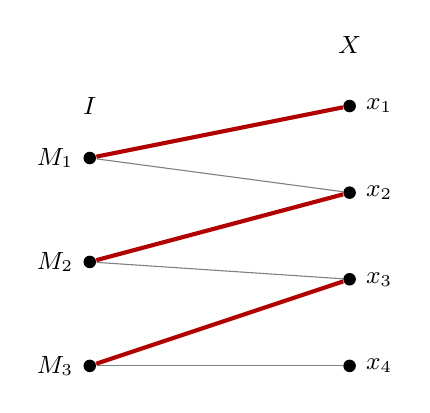
\begin{tikzpicture}[scale=1.1,vert/.style={circle,fill=black,inner sep=1.6pt},font=\small]
  % I vlevo
  \foreach \i/\y in {1/2.4,2/1.2,3/0} {\node[vert,label=left:{$M_{\i}$}] (i\i) at (0,\y) {};}
  % X vpravo
  \foreach \x/\y in {1/3,2/2,3/1,4/0} {\node[vert,label=right:{$x_{\x}$}] (x\x) at (3,\y) {};}
  % hrany (clenstvi): M1={x1,x2}, M2={x2,x3}, M3={x3,x4}
  \draw[gray] (i1)--(x1); \draw[gray] (i1)--(x2);
  \draw[gray] (i2)--(x2); \draw[gray] (i2)--(x3);
  \draw[gray] (i3)--(x3); \draw[gray] (i3)--(x4);
  % parovani (SRR): M1-x1, M2-x2, M3-x3
  \draw[red!70!black,line width=1.5pt] (i1)--(x1);
  \draw[red!70!black,line width=1.5pt] (i2)--(x2);
  \draw[red!70!black,line width=1.5pt] (i3)--(x3);
  \node at (0,3) {$I$}; \node at (3,3.7) {$X$};
\end{tikzpicture}\obrpopis{Incidenční graf systému $M_1=\{x_1,x_2\}$, $M_2=\{x_2,x_3\}$, $M_3=\{x_3,x_4\}$. Červené párování velikosti $3$ dává SRR $f(1)=x_1,\ f(2)=x_2,\ f(3)=x_3$.}
\end{center}

\begin{veta}[Hallova věta]
SRR v konečném systému $\Mcal=(M_i:i\in I)$ existuje, právě když platí \emph{Hallova podmínka}
\[
\forall J\subseteq I:\quad \Big|\bigcup_{j\in J}M_j\Big|\ \ge\ |J|.
\]
\end{veta}

\video{https://www.youtube.com/watch?v=Ihr6gMx7b9c}{Wrath of Math, \emph{Hall's Theorem and Condition for Bipartite Matchings} (Hallova věta a~Hallova podmínka pro párování v~bipartitním grafu).}

\begin{intuice}
Podmínka je zjevně \emph{nutná}: každých $|J|$ množin musí dohromady obsahovat aspoň $|J|$ různých prvků, jinak z nich nelze vybrat $|J|$ různých reprezentantů. Hallova věta říká, že tato samozřejmá nutná podmínka je i \emph{postačující} -- to je její netriviální obsah. Postačitelnost dokážeme elegantně \emph{přes toky}: hledání SRR převedeme na hledání maximálního toku v~síti. Párování velikosti~$|I|$ odpovídá toku velikosti~$|I|$ ze zdroje do stoku, a Hallova podmínka přesně zaručí, že \emph{každý} řez je velký (alespoň $|I|$) -- takže i maximální tok je velký a celé $I$ nasytí.
\end{intuice}

\begin{proof}[Princip důkazu.]
\textbf{Nutnost.} Je-li $f$ SRR, pak $\bigcup_{j\in J}M_j\supseteq\{f(j):j\in J\}$ a prvky $f(j)$ jsou navzájem různé, takže $\big|\bigcup_{j\in J}M_j\big|\ge|J|$.

\smallskip
\textbf{Postačitelnost} (přes toky v sítích), ve čtyřech krocích:
\begin{enumerate}[label=(\arabic*)]
  \item \textbf{Síť.} Z incidenčního grafu $B_{\Mcal}$ uděláme síť (viz obrázek níže): přidáme zdroj $z$ s hranami $z\to i$ pro každé $i\in I$, ponecháme hrany $i\to x$ pro $x\in M_i$ a přidáme hrany $x\to s$ do stoku $s$ pro každé $x\in X$. Všem hranám dáme kapacitu $1$.
  \item \textbf{Tok $=$ párování.} Celočíselný tok velikosti $t$ odpovídá párování velikosti $t$ v $B_{\Mcal}$: hrana $i\to x$, po níž teče jednotka, je párovací hrana, a jednotkové kapacity zaručí, že každé $i$ i každé $x$ je nejvýše v jedné. Maximální (celočíselný) tok najde Fordův--Fulkersonův algoritmus.
  \item \textbf{Každý řez má velikost $\ge|I|$.} U minimálního řezu lze předpokládat, že přetíná jen hrany $z\to i$ a $x\to s$ (kdyby přetínal nějakou hranu $i\to x$, lze ji nahradit hranou $z\to i$ na téže cestě, aniž se řez zvětší). Označme $A\subseteq I$ vrcholy, jejichž hrana $z\to i$ přeťatá \emph{není}. Pak řez obsahuje $|I|-|A|$ hran $z\to i$ (pro $i\notin A$) a -- aby z $A$ nic neproteklo do stoku -- všechny hrany $x\to s$ pro $x\in\bigcup_{i\in A}M_i$. Proto
    \[
    \text{velikost řezu}\ \ge\ (|I|-|A|)+\Big|\bigcup_{i\in A}M_i\Big|\ \ge\ (|I|-|A|)+|A|\ =\ |I|,
    \]
    kde prostřední nerovnost je právě Hallova podmínka pro $J=A$.
  \item \textbf{Závěr.} Podle věty o maximálním toku a minimálním řezu je maximální tok roven nejmenšímu řezu, tedy $\ge|I|$ (a zároveň $\le|I|$, víc ze zdroje nevyteče). Maximální tok má tak velikost $|I|$ -- to je párování nasycující celé $I$, a podle lemmatu výše je to hledaný SRR.
\end{enumerate}
\end{proof}

\begin{center}
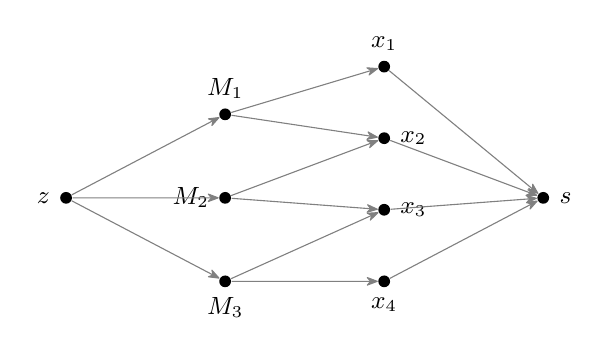
\begin{tikzpicture}[scale=1.01,>={Stealth[round]},vert/.style={circle,fill=black,inner sep=1.5pt},font=\small]
  \node[vert,label=left:{$z$}] (z) at (0,1.65) {};
  \node[vert,label=above:{$M_1$}] (i1) at (2,2.7) {};
  \node[vert,label=left:{$M_2$}] (i2) at (2,1.65) {};
  \node[vert,label=below:{$M_3$}] (i3) at (2,0.6) {};
  \node[vert,label=above:{$x_1$}] (x1) at (4,3.3) {};
  \node[vert,label=right:{$x_2$}] (x2) at (4,2.4) {};
  \node[vert,label=right:{$x_3$}] (x3) at (4,1.5) {};
  \node[vert,label=below:{$x_4$}] (x4) at (4,0.6) {};
  \node[vert,label=right:{$s$}] (s) at (6,1.65) {};
  \draw[->,gray] (z)--(i1); \draw[->,gray] (z)--(i2); \draw[->,gray] (z)--(i3);
  \draw[->,gray] (i1)--(x1); \draw[->,gray] (i1)--(x2);
  \draw[->,gray] (i2)--(x2); \draw[->,gray] (i2)--(x3);
  \draw[->,gray] (i3)--(x3); \draw[->,gray] (i3)--(x4);
  \draw[->,gray] (x1)--(s); \draw[->,gray] (x2)--(s); \draw[->,gray] (x3)--(s); \draw[->,gray] (x4)--(s);
\end{tikzpicture}\obrpopis{Síť pro důkaz Hallovy věty (systém $M_1=\{x_1,x_2\}$, $M_2=\{x_2,x_3\}$, $M_3=\{x_3,x_4\}$ z~obrázku výše): $z\to I\to X\to s$, všechny kapacity~$1$. Celočíselný tok velikosti $|I|$ je párování nasycující~$I$, tj.\ SRR.}
\end{center}

\begin{poznamka}
Předvedený důkaz je zároveň \emph{algoritmem}: SRR (resp.\ maximální párování) najde Fordův--Fulkersonův algoritmus v \textbf{polynomiálním} čase. Síť má jednotkové kapacity, takže každé hledání zlepšující cesty zvětší tok o $1$; cest je nejvýše $|I|$ a každá se najde prohledáním grafu (BFS/DFS) v čase $O(|E|)$. Celkem $O(|I|\cdot|E|)$ -- polynom ve velikosti vstupu. (Konstrukci sítě i větu o maximálním toku a minimálním řezu podrobně rozebírá okruh M4 -- toky v sítích; Hallovu větu lze dokázat i přímo indukcí nebo z Tutteovy věty, tok ale navíc dává konstruktivní algoritmus.)
\end{poznamka}

\begin{priklad}[Použití Hallovy věty]
\textbf{Zadání.}
\begin{enumerate}[label=(\arabic*)]
  \item Pro systém $M_1=\{1,2\}$, $M_2=\{2,3\}$, $M_3=\{1,3\}$ ověřte Hallovu podmínku a najděte SRR.
  \item Ukažte, že systém $M_1=M_2=M_3=\{1,2\}$ žádný SRR nemá.
\end{enumerate}

\textbf{Řešení.}
\begin{enumerate}[label=(\arabic*)]
  \item Stačí ověřit sjednocení pro všechny $J\subseteq I$: jednoprvkové dají $|M_i|=2\ge1$; každá dvojice dá $M_i\cup M_j=\{1,2,3\}$, tj.\ $3\ge2$; celé $M_1\cup M_2\cup M_3=\{1,2,3\}$ má velikost $3\ge3$. Hallova podmínka platí, SRR tedy existuje -- například $f(1)=1,\ f(2)=2,\ f(3)=3$ (různí reprezentanti, $f(i)\in M_i$).
  \item Pro $J=\{1,2,3\}$ je $\big|\bigcup_{j\in J}M_j\big|=|\{1,2\}|=2<3=|J|$. Hallova podmínka neplatí, takže SRR neexistuje: tři množiny by potřebovaly tři navzájem různé reprezentanty, ale dohromady nabízejí jen dva prvky.
\end{enumerate}
\end{priklad}

\begin{dusledek}[Postačující podmínka přes stupně]
Je-li v bipartitním grafu $B=(V_1\cup V_2,E)$ s neprázdnou množinou hran pro každé dva vrcholy $x\in V_1$, $y\in V_2$ splněno $\deg_B x\ge\deg_B y$, pak existuje párování nasycující $V_1$.
\end{dusledek}

\begin{intuice}
Položíme $M_i=$ sousedé vrcholu $i\in V_1$. Pro $J\subseteq V_1$ a $B(J)=\bigcup_{i\in J}M_i$ je počet hran mezi $J$ a $B(J)$ alespoň $|J|\cdot\min\deg$ a nejvýše $|B(J)|\cdot\max\deg$; z předpokladu $\min_{V_1}\deg\ge\max_{V_2}\deg$ pak plyne $|J|\le|B(J)|$, tedy Hallova podmínka. (Důsledkem je např.\ tvrzení, že každý \emph{latinský obdélník} $k\times n$ s $k<n$ lze doplnit na latinský čtverec $n\times n$.)
\end{intuice}

% ============================================================
\section*{Shrnutí}
\addcontentsline{toc}{section}{Shrnutí}

\begin{poznamka}
\textbf{Klíčové vlastnosti a vzorce (přehled k~SZZ).} Stručný výčet klíčových definic, vět a vzorců okruhu M3. Zkratky: ČUM $=$ částečně uspořádaná množina, SRR $=$ systém různých reprezentantů.

\smallskip
\emph{Vlastnosti binárních relací.}
\begin{itemize}
  \item Relace $R$ na $X$: \emph{reflexivní} $\forall x\colon xRx$; \emph{symetrická} $xRy\Rightarrow yRx$; \emph{antisymetrická} $(xRy\wedge yRx)\Rightarrow x=y$; \emph{tranzitivní} $(xRy\wedge yRz)\Rightarrow xRz$.
  \item Antisymetrie (slabá) povoluje smyčky -- zakazuje jen obousměrné hrany mezi \emph{různými} vrcholy. Asymetrie (ostrá) zakáže navíc smyčky (je ireflexivní).
  \item Složení $R\circ S=\{(x,z):\exists y,\ xRy\wedge ySz\}$; inverzní $R^{-1}=\{(y,x):(x,y)\in R\}$.
\end{itemize}

\smallskip
\emph{Ekvivalence a rozklady.}
\begin{itemize}
  \item \emph{Ekvivalence} $=$ refl.\ $+$ sym.\ $+$ trans. Třída prvku $x$: $[x]_R=\{y:xRy\}$.
  \item Ekvivalence na $X$ $\iff$ rozklady $X$ (třídy disjunktní, pokrývají $X$) -- 1:1 korespondence.
  \item Počet ekvivalencí na $n$-prvkové $X$ $=$ počet rozkladů $n$-prvkové množiny. Pro $n{=}4$: rozbor tvarů $4;\ 3{+}1;\ 2{+}2;\ 2{+}1{+}1;\ 1{+}1{+}1{+}1$ dá $1+4+3+6+1=15$.
\end{itemize}

\smallskip
\emph{Částečná uspořádání.}
\begin{itemize}
  \item \emph{Uspořádání} $=$ refl.\ $+$ antisym.\ $+$ trans.; \emph{lineární} (úplné): navíc každé dva porovnatelné. Příklady: $(\mathbb{R},\le)$ lineární; $(2^X,\subseteq)$, $(\mathbb{N},\mid)$ jen částečná.
  \item \emph{Minimální} prvek: nic pod ním (neexistuje $t$ s $t<a$). \emph{Nejmenší}: menší nebo roven \emph{všem} ($\forall x: a\le x$). Nejmenší $\Rightarrow$ minimální; opačně ne. Nejmenší je nejvýše jeden; minimálních může být více.
  \item \emph{Řetězec}: každé dva prvky porovnatelné. \emph{Antiřetězec}: žádné dva různé porovnatelné. \emph{Výška} $v$ $=$ délka nejdelšího řetězce; \emph{šířka} $s$ $=$ velikost největšího antiřetězce.
  \item \textbf{Věta o dlouhém a širokém}: $|X|\le v\cdot s$. Důkaz: rozvrstvit na patra minimálních prvků -- každé patro je antiřetězec ($\le s$ prvků), pater je $\le v$ (prvek $k$-tého patra leží v řetězci délky $k$).
  \item Erdős--Szekeres: v posloupnosti $n^2{+}1$ různých čísel existuje rostoucí nebo klesající podposloupnost délky $\ge n{+}1$ (ČUM na indexech: řetězec $=$ rostoucí, antiřetězec $=$ klesající, $n^2{+}1\le v\cdot s$).
\end{itemize}

\smallskip
\emph{Funkce: typy a počty.}
\begin{itemize}
  \item \emph{Prostá (injekce)}: $f(a)=f(b)\Rightarrow a=b$. \emph{Na (surjekce)}: $\forall y\in Y\ \exists x\in X:f(x)=y$. \emph{Bijekce}: prostá i na.
  \item Počty $f\colon A\to B$, $|A|=a$, $|B|=b$: \emph{všech} $b^a$; \emph{prostých} $\frac{b!}{(b-a)!}$ (pro $a\le b$, jinak $0$); \emph{bijekcí} $a!$ (jen $a=b$, jinak $0$); \emph{surjekcí} viz inkluze-exkluze níže.
  \item Speciálně: $k$-prvkových podmnožin $n$-prvkové $X$ je $\binom{n}{k}$; všech podmnožin $2^n$; permutací $n!$.
\end{itemize}

\smallskip
\emph{Permutace a pevný bod.}
\begin{itemize}
  \item Permutace $[n]$ $=$ bijekce $[n]\to[n]$; celkem $n!=n(n-1)\cdots1$ permutací. \emph{Pevný bod}: $p(x)=x$.
  \item Permutace bez pevného bodu (šatnářka): $D(n)=n!\sum_{k=0}^{n}\frac{(-1)^k}{k!}$; pravděpodobnost $\frac{D(n)}{n!}\to e^{-1}\approx0{,}368$ pro $n\to\infty$, skoro nezávislá na $n$.
\end{itemize}

\smallskip
\emph{Kombinační čísla a binomická věta.}
\begin{itemize}
  \item $\binom{n}{k}=\frac{n!}{k!\,(n-k)!}$ = počet $k$-prvkových podmnožin $n$-prvkové $X$. Symetrie: $\binom{n}{k}=\binom{n}{n-k}$. Pascal: $\binom{n}{k}=\binom{n-1}{k-1}+\binom{n-1}{k}$.
  \item Součty: $\sum_{k=0}^{n}\binom{n}{k}=2^n$; $\sum_{k=0}^{n}(-1)^k\binom{n}{k}=0$ (pro $n\ge1$; sudých podmnožin je stejně jako lichých).
  \item \emph{Binomická věta}: $(a+b)^n=\sum_{k=0}^{n}\binom{n}{k}a^{n-k}b^k$. Dosazením $a{=}b{=}1$ dostaneme $2^n$; $a{=}1$, $b{=}{-1}$ dostaneme $0$.
\end{itemize}

\smallskip
\emph{Princip inkluze a exkluze.}
\begin{itemize}
  \item Obecná formulace: $\bigl|\bigcup_{i=1}^{n}A_i\bigr|=\sum_{\emptyset\ne I\subseteq[n]}(-1)^{|I|-1}\bigl|\bigcap_{i\in I}A_i\bigr|$.
  \item Počítací důkaz: prvek v právě $j$ množinách přispěje $\sum_{k=1}^{j}(-1)^{k-1}\binom{j}{k}=1$.
  \item Šatnářka: $D(n)=n!\sum_{k=0}^{n}\frac{(-1)^k}{k!}$ (permutace bez pevného bodu; $A_i=\{\pi:\pi(i)=i\}$, $|A_i|=(n-1)!$).
  \item Eulerova funkce: $\varphi(n)=n\prod_{p\mid n}\bigl(1-\tfrac{1}{p}\bigr)$ = počet $m\le n$ s $\gcd(m,n)=1$; pro $n=p_1^{\alpha_1}\cdots p_r^{\alpha_r}$ a $A_i=\{m\le n:p_i\mid m\}$.
  \item Počet surjekcí $A\to B$: $\sum_{k=0}^{b}(-1)^k\binom{b}{k}(b-k)^a$ (pro $b^a$ všech funkcí odečteme ty, co vynechají aspoň jeden prvek $B$).
\end{itemize}

\smallskip
\emph{Hallova věta a SRR.}
\begin{itemize}
  \item \emph{SRR} systému $\Mcal=(M_i:i\in I)$: prostá $f\colon I\to X$ s~$f(i)\in M_i$ pro všechna $i$; ekvivalentní párování velikosti $|I|$ v incidenčním bipartitním grafu.
  \item \textbf{Hallova věta}: SRR existuje $\iff$ \emph{Hallova podmínka}: $\forall J\subseteq I:\ \bigl|\bigcup_{j\in J}M_j\bigr|\ge|J|$ (každých $|J|$ množin má dohromady $\ge|J|$ prvků).
  \item Princip důkazu (postačitelnost): síť $z\to I\to X\to s$, kapacity~$1$; tok velikosti $|I|$ $=$ SRR; každý řez $\ge|I|$ z Hallovy podmínky; max-tok $=$ min-řez $\Rightarrow$ tok velikosti $|I|$ existuje.
  \item Polynomiální algoritmus: Ford--Fulkerson v síti s jednotkovými kapacitami, čas $O(|I|\cdot|E|)$.
\end{itemize}
\end{poznamka}

% ============================================================
\section*{Zdroje}
\addcontentsline{toc}{section}{Zdroje}

{\raggedright
\begin{itemize}
  \item T.~Sláma: \emph{Diskrétní matematika}, zápisky z~přednášky NDMI002 (přednášející M.~Mareš), MFF UK, 2019/20 (primární zdroj výkladu relací, uspořádání, počítání a inkluze a exkluze).\\ \url{https://slama.dev/poznamky/diskretni-matematika/}
  \item J.~Matoušek, J.~Nešetřil: \emph{Kapitoly z~diskrétní matematiky}, Karolinum; anglicky \emph{Invitation to Discrete Mathematics}, 2.~vydání, Oxford University Press, 2008 (učebnice k~oběma předmětům; aplikace inkluze a exkluze, SRR).
  \item T.~Valla, J.~Matoušek: \emph{Kombinatorika a grafy I}, skripta, MFF UK, 2008 (kap.~4: systémy různých reprezentantů a Hallova věta).\\ \url{https://iuuk.mff.cuni.cz/~valla/kg.html}
  \item M.~Mareš: \emph{Kombinatorika do kapsy}, MFF UK, 2022 (kombinační čísla a binomická věta).\\ \url{https://mj.ucw.cz/papers/komb-tahak.pdf}
  \item Wrath of Math: \emph{Hall's Theorem and Condition for Bipartite Matchings} (video odkazované v~textu).\\ \url{https://www.youtube.com/watch?v=Ihr6gMx7b9c}
  \item MFF UK: požadavky ke státní závěrečné zkoušce (Informatika, Bc.) a zadání otázek z~minulých termínů.\\ \url{https://www.mff.cuni.cz/cs/studenti/bakalarske-studium/statni-zaverecne-zkousky/bakalarske-statni-zkousky-studijniho-programu-informatika}
\end{itemize}
\par}

\end{document}
